\documentclass[journal]{IEEEtran}
\usepackage{graphicx,amsmath,amssymb,booktabs,array,url,xcolor,multirow,cite}
\usepackage[T1]{fontenc}
\usepackage[utf8]{inputenc}
\usepackage{microtype}
\newcommand{\mainAUROC}{0.835 $\pm$ 0.041}
\newcommand{\mainAUPRC}{0.652 $\pm$ 0.028}
\newcommand{\mainFone}{0.567 $\pm$ 0.018}
\newcommand{\mainSens}{0.726 $\pm$ 0.082}
\newcommand{\mainFop}{0.731 $\pm$ 0.036}
\newcommand{\mainAUROCmin}{0.741}
\newcommand{\mainAUROCmax}{0.878}
\newcommand{\mainMACs}{11.1}
\newcommand{\mainParams}{42,483}
\newcommand{\nSeeds}{10}
\newcommand{\randAUROC}{0.835 $\pm$ 0.024}
\newcommand{\summaryAUROC}{0.674 $\pm$ 0.020}
\newcommand{\rrAUROC}{0.718 $\pm$ 0.018}
\newcommand{\pcNormal}{0.863}
\newcommand{\pcSVEB}{0.681}
\newcommand{\pcVEB}{0.961}
\newcommand{\rrSVEB}{0.441}
\newcommand{\rrVEB}{0.814}
\newcommand{\rrNormal}{0.901}
\newcommand{\afibN}{610}
\newcommand{\afibSens}{0.770 $\pm$ 0.127}
\newcommand{\otherSens}{0.714 $\pm$ 0.077}
\newcommand{\cnnAUROC}{0.809 $\pm$ 0.036}
\newcommand{\cnnMACs}{0.59}
\newcommand{\cnnParams}{4,563}
\newcommand{\tfoneAUROC}{0.826 $\pm$ 0.023}
\newcommand{\tfoneMACs}{5.85}
\newcommand{\tfoneParams}{23,523}
\newcommand{\noregAUROC}{0.816 $\pm$ 0.046}
\newcommand{\noregMACs}{11.11}
\newcommand{\noregParams}{42,483}
\newcommand{\norateAUROC}{0.821 $\pm$ 0.038}
\newcommand{\norateMACs}{11.11}
\newcommand{\norateParams}{42,483}
\newcommand{\noeeAUROC}{0.810 $\pm$ 0.052}
\newcommand{\noeeMACs}{11.11}
\newcommand{\noeeParams}{42,483}
\newcommand{\taskonlyAUROC}{0.780 $\pm$ 0.104}
\newcommand{\taskonlyMACs}{11.11}
\newcommand{\taskonlyParams}{42,483}
\newcommand{\mliiAUROC}{0.833 $\pm$ 0.041}
\newcommand{\mliiMACs}{11.0}
\newcommand{\fsTwoFiftyAUROC}{0.811 $\pm$ 0.051}
\newcommand{\fsTwoFiftyMACs}{31.5}
\newcommand{\fsThreeSixtyAUROC}{0.776 $\pm$ 0.038}
\newcommand{\fsThreeSixtyMACs}{57.2}
\newcommand{\taskNativeSixteen}{0.838 $\pm$ 0.021}
\newcommand{\taskLogregSixteen}{0.812 $\pm$ 0.021}
\newcommand{\taskNativeThirtyTwo}{0.840 $\pm$ 0.022}
\newcommand{\sameencSixteen}{0.642 $\pm$ 0.039}
\newcommand{\convaeSixteen}{0.537 $\pm$ 0.053}
\newcommand{\jsccSixteen}{0.580 $\pm$ 0.035}
\newcommand{\sameencThirtyTwo}{0.654 $\pm$ 0.037}
\newcommand{\convaeThirtyTwo}{0.536 $\pm$ 0.054}
\newcommand{\jsccThirtyTwo}{0.581 $\pm$ 0.035}
\newcommand{\taskPeSixteen}{0.782 $\pm$ 0.022}
\newcommand{\taskPeThirtyTwo}{0.801 $\pm$ 0.033}
\newcommand{\mainPeAUROC}{0.825 $\pm$ 0.055}
\newcommand{\pcaThirtyTwo}{0.515}
\newcommand{\pcaOneTwentyEight}{0.501}
\newcommand{\summaryProof}{0.675}
\newcommand{\rrProof}{0.718}
\newcommand{\sameencMSE}{0.819 $\pm$ 0.008}
\newcommand{\sameencPRD}{90.5 $\pm$ 0.5}
\newcommand{\convaeMSE}{0.745 $\pm$ 0.005}
\newcommand{\convaePRD}{86.3 $\pm$ 0.3}
\newcommand{\jsccMSE}{0.755 $\pm$ 0.021}
\newcommand{\jsccPRD}{86.9 $\pm$ 1.2}
\newcommand{\ptqEight}{0.835 $\pm$ 0.041}
\newcommand{\ptqSix}{0.835 $\pm$ 0.041}
\newcommand{\ptqFour}{0.834 $\pm$ 0.041}
\newcommand{\ptqThree}{0.832 $\pm$ 0.038}
\newcommand{\ptqTwo}{0.721 $\pm$ 0.049}
\newcommand{\qatFour}{0.831 $\pm$ 0.034}
\newcommand{\qatThree}{0.812 $\pm$ 0.047}
\newcommand{\kNinety}{19}
\newcommand{\kNinetyNine}{29}
\newcommand{\cumTwo}{27}
\newcommand{\cumFour}{42}
\newcommand{\cumEight}{62}
\newcommand{\subTopTwo}{0.828 $\pm$ 0.040}
\newcommand{\subTopFour}{0.840 $\pm$ 0.047}
\newcommand{\subTopEight}{0.837 $\pm$ 0.039}
\newcommand{\subRandFour}{0.758 $\pm$ 0.027}
\newcommand{\subRandEight}{0.805 $\pm$ 0.039}
\newcommand{\subRandSixteen}{0.821 $\pm$ 0.044}
\newcommand{\latFourAUROC}{0.829 $\pm$ 0.029}
\newcommand{\latFourFone}{0.552 $\pm$ 0.029}
\newcommand{\latFourN}{10}
\newcommand{\latEightAUROC}{0.829 $\pm$ 0.018}
\newcommand{\latEightFone}{0.572 $\pm$ 0.020}
\newcommand{\latEightN}{5}
\newcommand{\dimMaxDrop}{0.003}
\newcommand{\dimMedianDrop}{0.000}
\newcommand{\dimNsens}{0}
\newcommand{\snrFour}{12.2}
\newcommand{\iidForty}{0.818 $\pm$ 0.036}
\newcommand{\fragForty}{0.804 $\pm$ 0.036}
\newcommand{\burstForty}{0.799 $\pm$ 0.035}
\newcommand{\iidTen}{0.832 $\pm$ 0.040}
\newcommand{\bscOnePct}{0.830 $\pm$ 0.038}
\newcommand{\bscTenPct}{0.786 $\pm$ 0.025}
\newcommand{\burstBscOnePct}{0.830 $\pm$ 0.039}
\newcommand{\eraseIidForty}{0.823 $\pm$ 0.049}
\newcommand{\eraseBurstForty}{0.804 $\pm$ 0.050}
\newcommand{\eraseZero}{0.834 $\pm$ 0.049}
\newcommand{\eraseBscTenPct}{0.796 $\pm$ 0.046}
\newcommand{\bleRaw}{1.32}
\newcommand{\zRaw}{13.66}
\newcommand{\bleFullForty}{2.78}
\newcommand{\bleFullHundred}{1.13}
\newcommand{\bleFullTwoHundred}{0.58}
\newcommand{\zFullForty}{2.95}
\newcommand{\zFullHundred}{1.30}
\newcommand{\bleCnnForty}{0.172}
\newcommand{\zCnnForty}{0.344}
\newcommand{\bleCnnFactor}{7.7}
\newcommand{\zCnnFactor}{39.7}
\newcommand{\bleFullHundredFactor}{1.2}
\newcommand{\zFullHundredFactor}{10.5}
\newcommand{\zFullFortyFactor}{4.6}
\newcommand{\bleAirRaw}{45.6}
\newcommand{\bleAirSem}{0.88}
\newcommand{\airFactor}{52}
\newcommand{\cpuCrossBLEms}{131}
\newcommand{\cpuCrossZms}{1360}
\newcommand{\crossMMAC}{85}
\newcommand{\pqEncapsMs}{6.1}
\newcommand{\pqVerifyMs}{22}
\newcommand{\pqNodeMJ}{0.35}
\newcommand{\pqNodeMs}{35}
\newcommand{\pqKeygenMs}{6.1}
\newcommand{\pqSignMs}{62}
\newcommand{\pqDecapsMs}{6.7}
\newcommand{\ptbxlAUROC}{0.920 $\pm$ 0.004}
\newcommand{\ptbxlAUPRC}{0.948 $\pm$ 0.002}
\newcommand{\ptbxlFone}{0.830 $\pm$ 0.006}
\newcommand{\ptbxlNtest}{2,158}
\newcommand{\ptbxlNtrain}{17,076}
\newcommand{\ptbxlNval}{2,144}
\newcommand{\ptbxlNrec}{21,378}
\newif\ifhavepe \havepetrue
\newif\ifhavelat \havelattrue
\newcommand{\latConfirmSentence}{Training codecs with $D=8$ and $D=4$ from scratch confirms it (Table~\ref{tab:quant}): 0.829 $\pm$ 0.018 and 0.829 $\pm$ 0.029, indistinguishable from the 32-coefficient codec.}
\newif\ifhaveptbxl \haveptbxltrue
\newcommand{\ptbxlRow}{PTB-XL, 12 leads, NORM vs.\ abnormal & 0.920 $\pm$ 0.004 & 0.948 $\pm$ 0.002 & 0.830 $\pm$ 0.006 \\}

\newcommand{\bz}{\mathbf{z}}
\newcommand{\bx}{\mathbf{x}}
\newcommand{\bq}{\mathbf{q}}
\newcommand{\R}{\mathbb{R}}

\begin{document}
\title{Task-Oriented Semantic Coding for Energy-Efficient and Post-Quantum-Secure Wearable ECG Telemetry}
\author{Mustafa~A.~Azzawi%
\thanks{M. A. Azzawi is an independent researcher, New York, NY, USA (e-mail: mazzawi1991@gmail.com). ORCID 0000-0002-9360-4174.}%
\thanks{Code, trained-result files, and the scripts that regenerate every table and figure are available at \texttt{github.com/azzawi91/task-oriented-semantic-ecg}.}}
\markboth{IEEE Transactions on Green Communications and Networking}{Azzawi: Task-Oriented Semantic Coding for Energy-Efficient and Post-Quantum-Secure Wearable ECG Telemetry}
\maketitle

\begin{abstract}
The radio, not the processor, sets the energy budget of a battery-powered wearable electrocardiogram (ECG) node, yet most transmitted samples never change the clinical decision. This article treats task-oriented semantic coding for wearable ECG as a green-communication problem: a compact on-device encoder (\mainParams{} parameters) maps each 10-s window to a 32-coefficient latent, quantized to $b$ bits and sealed by authenticated encryption, and an edge gateway decodes it directly into an arrhythmia decision. On the patient-disjoint DS1/DS2 partition of the MIT-BIH Arrhythmia Database the codec reaches an AUROC of \mainAUROC{} over \nSeeds{} seeds with a 60-byte payload, 98.8\% below the 5000-byte raw window. Matched-payload comparisons against reconstruction codecs\ifhavepe{} (including one with the identical encoder)\fi{} and against PCA, spectral-summary, and RR-interval codes isolate the training objective as the source of the gain: at 16 bytes the task-trained latent retains \taskNativeSixteen{}, whereas \ifhavepe the same architecture trained for reconstruction retains \sameencSixteen{}\else the reconstruction codecs retain \convaeSixteen{} and \jsccSixteen{}\fi. Post-training quantization is lossless down to 3 bits per coefficient, \ifhavelat a 4-coefficient codec retains \latFourAUROC{} with a 4-byte code, \else the four highest-variance coefficients alone retain \subTopFour{}, \fi and the 28-byte authenticated-encryption overhead becomes the payload floor. An energy model that counts attention operations explicitly places the compute--radio crossover of the full codec near \crossMMAC{}\,M~MAC/s on Bluetooth Low Energy, whereas a CNN-only variant (\cnnMACs{}\,M MACs per window, AUROC \cnnAUROC{}) and IEEE~802.15.4 links save energy unambiguously. Robustness to i.i.d.\ and bursty erasure and bit-flip channels, single-lead input, and 125--360~Hz sampling is evaluated, and the post-quantum layer (ML-KEM-512, ML-DSA-44) is costed from published Cortex-M4 cycle counts. All energy and security figures are model-based and are reported as such.
\end{abstract}

\begin{IEEEkeywords}
Semantic communication, task-oriented coding, green communications, wearable ECG, Internet of Medical Things, energy modeling, quantization, post-quantum cryptography.
\end{IEEEkeywords}

\section{Introduction}
\IEEEPARstart{C}{ontinuous} ambulatory ECG monitoring is the main tool for catching arrhythmias that short clinical recordings miss, and body-worn nodes of the Internet of Medical Things (IoMT) now stream cardiac signals to gateways and the cloud around the clock. The bottleneck of such a node is neither sensing nor computation but the wireless uplink: the radio dominates the energy budget, the body-area link offers limited and shared bandwidth, and fading and packet loss are routine. Conventional telemetry transmits the digitized waveform or a generic compression of it, both of which spend energy and airtime on samples that do not alter the decision made at the receiver, and a sample-distortion objective is indifferent to whether the morphology that signals an arrhythmia survives quantization and channel impairment.

Semantic and task-oriented communication conveys only what the receiver needs to accomplish its task \cite{strinati2021,gunduz2023,qin2022,yang2023,luo2022,getu2024}. Learned joint source--channel coding (JSCC) has shown for images \cite{bourtsoulatze2019}, text \cite{xie2021}, and speech \cite{weng2021} that a representation trained for the downstream objective tolerates aggressive compression and channel noise better than separate source and channel codes. Applied to physiological telemetry, the principle is to transmit a compact, decision-relevant representation of the ECG and let the gateway decode a diagnosis directly. Its transfer to wearable biosignals is still thin \cite{chen2024}: prior work rarely quantifies, on a recognized clinical benchmark under a leakage-free patient-disjoint protocol, how much coding for the task saves relative to coding for reconstruction, rarely accounts for the on-device computation that the encoder adds to the energy budget, and rarely addresses the long-lived confidentiality that medical data require against harvest-now, decrypt-later adversaries \cite{bernstein2017,alagic2022}.

\begin{figure*}[!t]
\centering
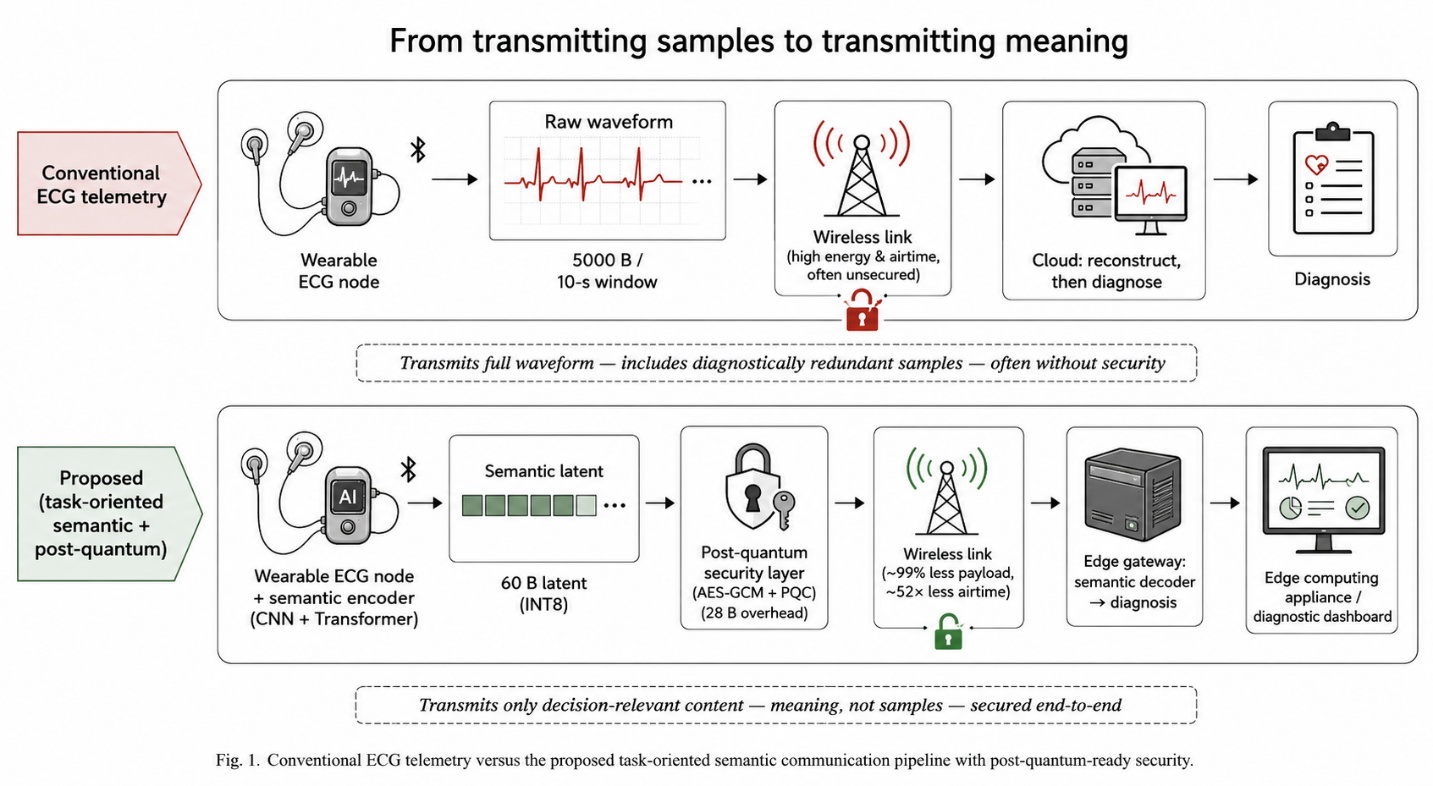
\includegraphics[width=0.6\textwidth]{figs/fig0_intro_concept.png}
\caption{Conventional versus task-oriented ECG telemetry. Raw transmission sends about 5000 bytes per 10-s window; the proposed node sends a 60-byte, authenticated latent that the gateway decodes directly into a decision. The trade this article quantifies is radio bytes and airtime against on-device encoder computation.}
\label{fig:concept}
\end{figure*}

This article treats task-oriented ECG coding as a green-communication design problem and answers the questions a deployment would raise. Which part of the model carries the diagnostic information, and how much computation is needed to preserve it? At what payload does a task-trained code outperform a reconstruction code trained with equal care? How does the code degrade under quantization to a few bits, under bursty erasures and bit errors, and does channel-aware training help? When does the encoder's computation exceed the radio energy it saves? What do standardized post-quantum primitives add to a 60-byte packet stream? The contributions are:
\begin{itemize}
\item a complete formulation of the codec (Section~\ref{sec:model}--\ref{sec:method}): encoder, straight-through quantizer, rate estimate, loss, channel, decoder, and the analytical link and energy model, with the full layer specification in the main text (Table~\ref{tab:arch});
\item a matched-payload comparison on the de Chazal partition against reconstruction codecs trained to convergence with validation-based selection, including a control with the identical encoder architecture, and against PCA, spectral-summary, and RR-interval codes (Section~\ref{sec:proof});
\item an ablation of the encoder and loss (Section~\ref{sec:ablation}) that identifies a CNN-only variant with 19$\times$ fewer MACs as the energy-efficient operating point, and single-lead and sampling-rate studies (Section~\ref{sec:input});
\item quantization analysis (post-training versus quantization-aware, per-coefficient sensitivity, error distribution) and channel robustness under i.i.d.\ and Gilbert--Elliott bursty erasure and bit-flip channels, with erasure-aware training (Sections~\ref{sec:quant}--\ref{sec:channel});
\item an energy model that counts attention MACs, reports the compute--radio crossover explicitly, and sweeps INT8 throughput, radio, and packet-error rate (Section~\ref{sec:energy}); and a post-quantum overhead analysis from FIPS 203/204 sizes and pqm4 Cortex-M4 cycle counts (Section~\ref{sec:security}).
\end{itemize}
All numbers reproduce from the released code. Energy and cryptographic costs are analytical, parameterized by datasheets and published benchmarks; no on-device measurement is claimed (Section~\ref{sec:discussion}).

\section{Related Work}
\subsection{Semantic and task-oriented communication}
Semantic communication reframes Shannon's reproduction problem \cite{shannon1948} toward conveying task utility \cite{strinati2021,gunduz2023}, a direction now broadly surveyed \cite{qin2022,yang2023,luo2022,getu2024}. Deep JSCC learns transmitter and receiver jointly \cite{bourtsoulatze2019,xie2021,weng2021}, and nonlinear-transform, feedback, and constellation-constrained variants advance its rate--distortion frontier \cite{dai2022,kurka2020,tung2022}; the entropy models used for rate estimation originate in learned image compression \cite{balle2017,balle2018}. This article specializes task-oriented coding to a wearable transmitter with tight energy and memory limits and measures, rather than assumes, the gap between coding for a decision and coding for reconstruction.

\subsection{Machine learning and compression for ECG}
Deep networks classify ECG at expert level \cite{hannun2019,ribeiro2020}; open benchmarks \cite{moody2001,goldberger2000,strodthoff2021,wagner2020} under the AAMI grouping \cite{aami2012} and the inter-patient partition of de Chazal et al.\ \cite{dechazal2004} standardize evaluation, and convolutional, recurrent, and attention models dominate recent arrhythmia work \cite{acharya2017,kachuee2018,mousavi2019,yildirim2018,xia2023,essa2021}. Waveform compression by autoencoders and compressed sensing \cite{yildirim2018c,mamaghanian2011} targets reconstruction fidelity, the objective that Section~\ref{sec:proof} shows to be a poor proxy for transmitting a decision. Classical arrhythmia detection from RR-interval statistics \cite{pan1985} provides the hand-crafted reference used here.

\subsection{Security, body-area networking, and on-device efficiency}
Confidentiality and integrity are first-order IoMT concerns \cite{frustaci2018,hatzivasilis2018}; post-quantum migration rests on the lattice schemes standardized as ML-KEM and ML-DSA \cite{fips203,fips204,bos2018,ducas2018} and benchmarked on microcontrollers by pqm4 \cite{pqm4}, with recent adaptations to constrained health devices \cite{bernstein2017,alagic2022} over authenticated record layers \cite{gcm,hkdf}. Wearable telemetry runs over IEEE~802.15.6 and 802.15.4 \cite{ieee802156,ieee802154} and Bluetooth Low Energy \cite{gomez2012,ble53}, surveyed for energy-efficient operation \cite{ullah2012,cavallari2014}; the energy model in Section~\ref{sec:energy} is parameterized by commodity radio datasheets \cite{nrf52840,cc2652r}. On-device intelligence relies on quantization and efficient kernels \cite{han2016,jacob2018,lai2018,banbury2021}; the compute--radio crossover analysed here connects that literature to the link budget.

\section{System Model and Problem Formulation}\label{sec:model}
\begin{figure*}[!t]
\centering
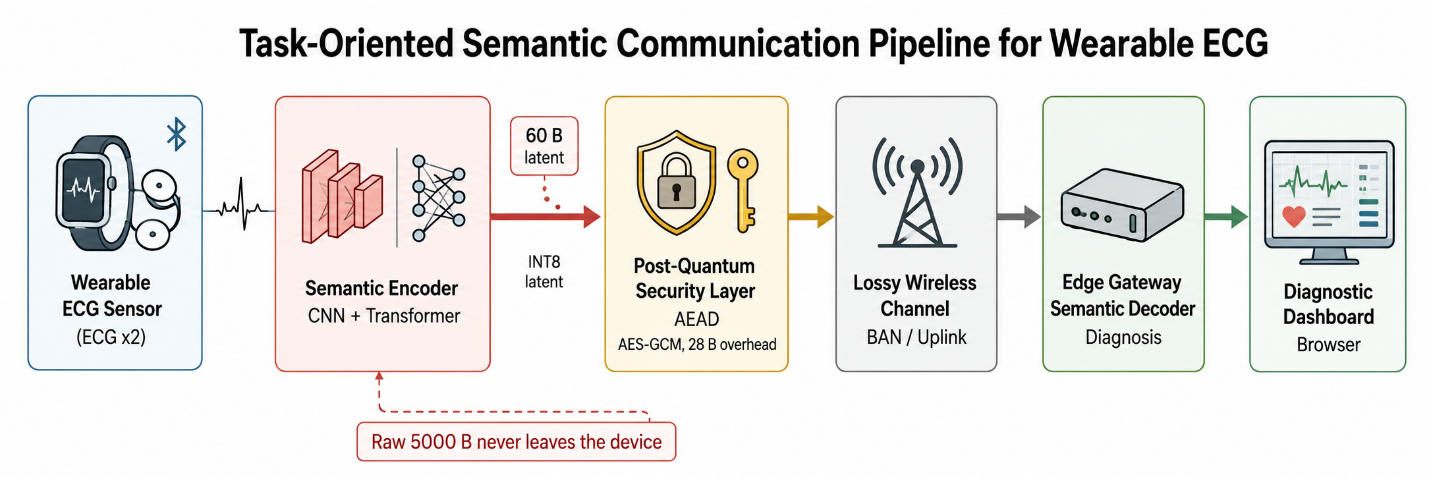
\includegraphics[width=0.6\textwidth]{figs/fig1_architecture.png}
\caption{System architecture. The wearable node encodes each ECG window into a 32-coefficient latent, quantizes it to $b$ bits, and seals it with the record layer; the gateway decodes the received latent into a class posterior. The raw window never leaves the device.}
\label{fig:arch}
\end{figure*}

\subsection{Signals, codec, and channel}
A wearable node samples $C$ ECG leads at $f_s$~Hz and forms non-overlapping windows $\bx\in\R^{C\times T}$ of $W=10$~s, $T=f_sW$, each z-scored per lead. Raw transmission costs $B_{\rm raw}=2CT$ bytes per window with 16-bit samples: 5000 bytes for $C=2$, $f_s=125$~Hz. The proposed node computes
\begin{equation}
\bz=f_\phi(\bx)\in\R^{D},\qquad \bq=Q_b(\bz)\in\{-2^{b-1},\dots,2^{b-1}-1\}^{D},
\label{eq:enc}
\end{equation}
with $D=32$ and a uniform symmetric quantizer $Q_b(z)=\mathrm{clip}(\mathrm{round}(z\,q_b),-q_b-1,q_b)$, $q_b=2^{b-1}-1$; the dequantized value is $\hat z=q/q_b$. The code costs $B_b=\lceil Db/8\rceil$ bytes and the transmitted payload is $B_b+28$ bytes after the 16-byte authentication tag and 12-byte nonce of the record layer (Section~\ref{sec:secmethod}). The channel maps $\bq$ to $\tilde{\bq}$ by erasing coefficients or fragments, or by flipping bits (Section~\ref{sec:channelmodel}); the gateway computes the posterior $p_\psi(y\,|\,\tilde{\bq})=g_\psi(\tilde{\bq}/q_b)$ over $K$ classes with a decoder $g_\psi$. The encoder and decoder are subject-independent: they are trained once on the training population, the encoder is shipped as node firmware and the decoder lives at the gateway, and no per-subject parameters are exchanged. The task is the AAMI EC57 window-level decision $y\in\{$normal, supraventricular ectopy (SVEB), ventricular ectopy (VEB)$\}$ \cite{aami2012}; binary abnormal-versus-normal operating points use the score $1-p_\psi(\text{normal}\,|\,\tilde{\bq})$. The node's actions per window are therefore fixed and few: encode, quantize at the current $b$, seal, transmit; $b$ is the only run-time control.

\subsection{Per-decision costs}
Three costs are tracked per decision. Payload $B$ (bytes) determines airtime $t_{\rm air}(B)$ on a given radio and, with the transmit current, the radio energy $E_{\rm tx}(B)$. Encoder computation adds $E_{\rm cpu}=P_{\rm cpu}\,M/\Theta$ for $M$ MACs at an INT8 throughput of $\Theta$ MAC/s and active power $P_{\rm cpu}$. Diagnostic fidelity is measured by macro one-versus-rest AUROC and AUPRC, macro-F1, and sensitivity at 90\% specificity with the threshold calibrated on held-out training records. The green design question is when $E_{\rm cpu}(M,\Theta)+E_{\rm tx}(B_b+28)<E_{\rm tx}(B_{\rm raw})$ holds while fidelity is preserved; Section~\ref{sec:energy} answers it as a function of $M$, $\Theta$, radio, and packet-error rate.

\subsection{Security model}
The adversary records ciphertext today and may later possess a cryptographically relevant quantum computer; it may also impersonate the gateway. The requirements are confidentiality of every latent, gateway authenticity, and per-packet integrity, at a per-decision overhead small relative to a 32-byte code.

\section{Method}\label{sec:method}
\subsection{Encoder and decoder}
Table~\ref{tab:arch} specifies the encoder for $C=2$, $f_s=125$~Hz. A stride-2 convolutional stem is followed by two depthwise-separable blocks \cite{howard2017,chollet2017} with GroupNorm and GELU, producing $L=157$ tokens of width $d=48$. A two-layer Transformer encoder \cite{vaswani2017} ($h=4$ heads, feed-forward width 96, dropout 0.1, GELU) mixes the tokens; mean pooling and a linear layer give $\bz$. No positional encoding is added: self-attention and the per-token feed-forward layers are permutation-equivariant and the mean pool is permutation-invariant, so $\bz$ is a function of the \emph{multiset} of context-mixed local tokens (each token sees about 0.25~s of signal) and is invariant to where in the window a beat occurs. This is deliberate for a decision code---the AAMI label does not depend on beat phase---and it is the property that principal-component coding lacks (Section~\ref{sec:proof}); it also means that this encoder cannot be trained to reconstruct a waveform\ifhavepe, which the control experiment of Section~\ref{sec:proof} accounts for by adding fixed sinusoidal positional encodings to both members of the compared pair\fi. An auxiliary early-exit head on the pooled feature is used only in training. The decoder $g_\psi$ is a two-hidden-layer perceptron (32--96--48--$K$, GELU). The encoder holds \mainParams{} parameters and needs \mainMACs{}\,M MACs per window; the count includes the attention projections and the $L\times L$ score and context products, which hook-based profilers omit because multi-head attention is a functional call---the 3.6\,M figure reported in an earlier version of this work counted only convolution and feed-forward layers. Section~\ref{sec:ablation} shows what the Transformer buys for that cost.

\begin{table}[!t]
\centering
\caption{Encoder specification (two leads, 125 Hz; 10-s window). Shapes are channels$\times$length or tokens$\times$width.}
\label{tab:arch}
\footnotesize
\resizebox{\columnwidth}{!}{\begin{tabular}{llrr}
\toprule
Stage & Layer & Output & Params \\
\midrule
Input & z-scored window & $2\times1250$ & -- \\
Stem & Conv1d $k$=7, $s$=2, 16 ch. & $16\times625$ & 240 \\
Block 1 & DW-Conv $k$=5, $s$=2; PW 16$\to$32; GN(4); GELU & $32\times313$ & 704 \\
Block 2 & DW-Conv $k$=5, $s$=2; PW 32$\to$48; GN(4); GELU & $48\times157$ & 1,872 \\
Transformer & 2 layers, $d$=48, 4 heads, FFN 96, LayerNorm & $157\times48$ & 37,920 \\
Pool + latent & mean over tokens; Linear 48$\to$32 & 32 & 1,568 \\
Aux.\ heads & early-exit Linear 48$\to$3; rate model $\log\sigma$ & -- & 179 \\
\midrule
Encoder total & & & 42,483 \\
Decoder & Linear 32$\to$96, GELU, Linear 96$\to$48, GELU, Linear 48$\to$3 & 3 & 7,971 \\
\bottomrule
\end{tabular}}
\end{table}

\subsection{Training objective}
Quantization is inside the training graph through a straight-through estimator \cite{bengio2013}: the forward pass uses $\hat\bz=Q_b(\bz)/q_b$ and the backward pass treats $Q_b$ as the identity, so the decoder is trained on exactly the codes it will receive. With decoder logits $g_\psi(\hat\bz)$, early-exit logits $\ell_{\rm ee}$, and the label $y$, the loss is
\begin{equation}
\mathcal{L}=\tfrac12\big[\mathrm{CE}(g_\psi(\hat\bz),y)+\mathrm{CE}(\ell_{\rm ee},y)\big]+\gamma\,\mathcal{R}(\hat\bz)+\lambda\,\|\hat\bz\|_2^2/D,
\label{eq:loss}
\end{equation}
where the rate surrogate is the code length under a factorized Gaussian prior with learned per-coefficient scales $\sigma_j$ \cite{balle2017},
\begin{equation}
\mathcal{R}(\hat\bz)=\frac{1}{D}\sum_{j=1}^{D}\Big[\frac{\hat z_j^2}{2\sigma_j^2}+\log\sigma_j+\tfrac12\log 2\pi\Big]\Big/\ln 2 \;\text{bits},
\end{equation}
and the $\ell_2$ term keeps the latent inside the quantizer range and acts as a variational-bottleneck surrogate (the KL divergence between $\mathcal N(\bz,I)$ and $\mathcal N(0,I)$ is $\|\bz\|^2/2$ \cite{tishby2015,alemi2017}). The weights are $\gamma=0.05$ and $\lambda=0.105$; the latter equals the sum of two $\ell_2$-type terms (KL surrogate $0.5\times0.01$ and magnitude penalty $0.10$) that were listed separately in the released configuration and are merged here because they are proportional. Training uses Adam \cite{kingma2015} at $3\times10^{-3}$, batch 64, six epochs, $b=8$ unless stated. The variant in Section~\ref{sec:channel} additionally zeroes each quantized coefficient with probability 0.2 during training (erasure-aware training), the latent-domain analogue of a JSCC channel layer.

\subsection{Rate adaptation and quantization}
Because the transmitted object is $\bq$, the bit-width $b$ sets the payload directly: 32, 24, 16, 12, and 8 bytes for $b=8,6,4,3,2$. Two ways of operating below 8 bits are compared: post-training quantization (PTQ), where the 8-bit-trained encoder's latent is requantized at the node, and quantization-aware training (QAT) \cite{jacob2018}, where the straight-through quantizer runs at the target $b$ throughout training. PTQ needs one model and lets the node track link quality without retraining; QAT needs one model per $b$.

\subsection{Channel models}\label{sec:channelmodel}
Four impairments are applied to the integer code $\bq$ at the receiver. (i) I.i.d.\ coefficient erasure with probability $\epsilon$ (an erased coefficient is set to zero, the prior mean). (ii) Fragment erasure: the 32 coefficients are split into four 8-coefficient fragments, modeling a payload that spans several link-layer packets, each lost with probability $\epsilon$ i.i.d. (iii) Bursty fragment erasure from a two-state Gilbert--Elliott chain \cite{gilbert1960,elliott1963} over successive fragments with bad-to-good transition probability $0.5$ and the good-to-bad probability chosen so that the stationary loss equals $\epsilon$. (iv) Bit errors on the two's-complement code: an i.i.d.\ binary symmetric channel with crossover $p$, and a bursty variant in which a Gilbert--Elliott chain over the coefficient sequence flips each bit of a coefficient with probability $0.1$ in the bad state and never in the good state, tuned to the same mean bit-error rate. Block Rayleigh fading with an SNR threshold maps to (ii)--(iii) through $\epsilon=1-\exp(-\gamma_{\rm th}/\bar\gamma)$ \cite{gomez2012}.

\subsection{Security layer}\label{sec:secmethod}
Each session starts with a handshake: the gateway's ML-DSA-44 public key (1312 B) is provisioned at pairing; the node generates an ML-KEM-512 key pair and sends the 800-byte encapsulation key, the gateway returns the 768-byte ciphertext and a 2420-byte ML-DSA-44 signature over the transcript, and the node verifies the signature and decapsulates. An HKDF schedule \cite{hkdf} derives directional AES-128-GCM keys \cite{gcm}; every latent is then sealed with a 12-byte nonce and 16-byte tag. Sizes are the FIPS 203/204 values \cite{fips203,fips204}; the node-side cost per session is one ML-KEM key generation, one decapsulation, and one signature verification, whose cycle counts are taken from pqm4 \cite{pqm4} (Section~\ref{sec:security}).

\subsection{Link and energy model}\label{sec:energymethod}
For a radio with bit rate $R$, maximum payload $m$ per packet, per-packet overhead $o$ bytes, inter-frame space $t_{\rm ifs}$, ramp time $t_{\rm r}$, transmit current $I_{\rm tx}$, and supply $V$, a $B$-byte payload needs $n=\lceil B/m\rceil$ packets,
\begin{equation}
t_{\rm air}=\frac{8(B+n\,o)}{R}+n\,t_{\rm ifs}+t_{\rm r},\qquad E_{\rm tx}=I_{\rm tx}V\,t_{\rm air},
\end{equation}
and with an ARQ packet-error rate $\rho$ the expected radio energy is $E_{\rm tx}/(1-\rho)$. The encoder costs $E_{\rm cpu}=I_{\rm cpu}V\,M/\Theta$. Parameters follow the nRF52840 (BLE 1M PHY: $R$=1~Mb/s, $m$=244, $o$=14, $I_{\rm tx}$=9.65~mA at 0~dBm) and CC2652R (IEEE~802.15.4: $R$=250~kb/s, $m$=116, $o$=15, $I_{\rm tx}$=24~mA) datasheets \cite{nrf52840,cc2652r}, $V$=3~V, $I_{\rm cpu}$=3.3~mA (Cortex-M4F at 64~MHz), and $\Theta\in\{40,100,200\}$~M~MAC/s spanning conservative to optimized CMSIS-NN INT8 kernels \cite{lai2018}. Battery life assumes a 220-mAh coin cell, one decision per 10~s, and counts only these active energies. The model is analytical; Section~\ref{sec:discussion} states what it omits.

\section{Experimental Setup}
\textbf{Data.} The MIT-BIH Arrhythmia Database \cite{moody2001,goldberger2000} (48 two-lead records, 360~Hz, expert beat and rhythm annotations) is resampled to 125~Hz (250 and 360~Hz in Section~\ref{sec:input}) and cut into 8147 labeled 10-s windows: 5134 normal, 620 SVEB, 2393 VEB, following AAMI EC57 (a window is VEB if it contains any ventricular ectopic beat, SVEB if it contains a supraventricular ectopic beat and no VEB, normal otherwise; windows containing only paced or unclassifiable beats are dropped). The rhythm annotation in effect at each window centre is retained so that pathological rhythms such as atrial fibrillation (AF) can be examined. PTB-XL \cite{wagner2020} (21,799 12-lead, 10-s, 100~Hz records with official stratified folds; NORM versus any other diagnostic superclass, records without a diagnostic statement excluded) and WESAD \cite{schmidt2018} (chest ECG at 700~Hz and wrist PPG at 64~Hz; binary stress) serve the transfer experiments.

\textbf{Protocols.} The primary protocol is the de Chazal partition \cite{dechazal2004}: DS1 (22 records) trains, DS2 (22 records, 3960 windows) tests, paced records 102, 104, 107, 217 are excluded, and four seeded DS1 records are held out to calibrate the operating point, so DS2 is never touched by model or threshold selection. Ten seeds vary initialization, batch order, and calibration records; DS2 is fixed. A random record-disjoint 60/20/20 split (three seeds) is the secondary protocol. PTB-XL uses folds 1--8/9/10 for train/validation/test (five seeds); WESAD uses a subject-disjoint 9/3/3 split (five seeds).

\textbf{Baselines.} All codes are read by one logistic-regression head (class-balanced, $L_2$, 3000 iterations) fitted on the training-split codes, so differences reflect the representation. Reconstruction codecs with a 32-coefficient bottleneck are trained on DS1 to minimize waveform mean-squared error (MSE): (a) a convolutional autoencoder (encoder Conv1d $k$=7/5/5, stride 4, 16/32/48 channels, GELU, Linear 960$\to$32; mirrored transposed-convolution decoder); (b) the same autoencoder trained as a deep JSCC with additive white Gaussian noise at 10~dB on the code\ifhavepe; (c) the task encoder of Table~\ref{tab:arch} with fixed sinusoidal positional encodings added to the tokens (without them the order-invariant latent cannot represent phase and the reconstruction loss stays at its trivial value of 1.0), followed by a transposed-convolution decoder (Linear 32$\to$48$\times$157, three ConvTranspose1d stages); the task model is also retrained with the same positional encodings so that the pair differs only in the objective\fi. Codecs (a)--(b) train for 60 epochs\ifhavepe{} and (c) for 30\fi, Adam at $2\times10^{-3}$ with cosine decay, batch 64, three seeds, and the epoch with the lowest validation MSE is kept. Their codes are scaled per coefficient by the 99.9th percentile of the training latent before quantization, a fixed codec parameter, so that no code is clipped. Linear codes are PCA of the raw window (16--128 coefficients), a 22-coefficient spectral-summary code (per lead: mean, standard deviation, RMS, and eight low-frequency FFT magnitudes), and a 22-coefficient RR-interval code built from a Pan--Tompkins-style detector \cite{pan1985} (RR mean, SD, RMSSD, pNN50, extrema, coefficient of variation, median absolute deviation, beat rate, R-amplitude statistics, and eight tachogram spectral bins).

\textbf{Metrics and reproducibility.} AUROC and AUPRC are macro one-versus-rest; macro-F1 uses the arg-max decision; sensitivity at 90\% specificity and the operating-point F1 use the calibrated threshold. Means and standard deviations are over seeds. The pipeline is CPU-only PyTorch; caches, splits, and every table and figure regenerate from the released scripts.

\section{Results}
\subsection{Diagnostic accuracy}\label{sec:accuracy}
\begin{table*}[!t]
\centering
\caption{Diagnostic performance on the fixed DS2 test set (de Chazal protocol, \nSeeds{} seeds) and under the random record-disjoint split. Classical codes are read by logistic regression from 8-bit quantized 22-coefficient codes.}
\label{tab:main}
\footnotesize
\resizebox{\textwidth}{!}{\begin{tabular}{lccccc}
\toprule
Model / protocol & AUROC & AUPRC & Macro-F1 & Sens.@90\%Spec. & F1@op \\
\midrule
Spectral-summary code + logistic regression (22 B) & 0.674 $\pm$ 0.020 & -- & 0.432 $\pm$ 0.021 & -- & -- \\
RR-interval code + logistic regression (22 B) & 0.718 $\pm$ 0.018 & -- & 0.539 $\pm$ 0.023 & -- & -- \\
Task-oriented codec, de Chazal DS1/DS2 (10 seeds) & 0.835 $\pm$ 0.041 & 0.652 $\pm$ 0.028 & 0.567 $\pm$ 0.018 & 0.726 $\pm$ 0.082 & 0.731 $\pm$ 0.036 \\
Task-oriented codec, random record-disjoint (3 seeds) & 0.835 $\pm$ 0.024 & 0.609 $\pm$ 0.027 & 0.474 $\pm$ 0.101 & 0.638 $\pm$ 0.116 & 0.704 $\pm$ 0.062 \\
\bottomrule
\end{tabular}
}
\end{table*}
\begin{table}[!t]
\centering
\caption{Per-class discrimination on DS2 and sensitivity of the calibrated operating point on windows annotated as atrial fibrillation or flutter.}
\label{tab:perclass}
\small
\resizebox{\columnwidth}{!}{\begin{tabular}{lccc}
\toprule
Class (one-vs-rest AUROC on DS2) & Task-oriented codec & Spectral-summary code & RR-interval code \\
\midrule
Normal & 0.863 $\pm$ 0.038 & 0.670 & 0.901 \\
Supraventricular (SVEB) & 0.681 $\pm$ 0.092 & 0.621 & 0.441 \\
Ventricular (VEB) & 0.961 $\pm$ 0.010 & 0.731 & 0.814 \\
\midrule
Sensitivity at the calibrated operating point, windows in AF/AFL rhythm ($n$=610) & 0.770 $\pm$ 0.127 & -- & -- \\
Sensitivity at the calibrated operating point, all other abnormal windows & 0.714 $\pm$ 0.077 & -- & -- \\
\bottomrule
\end{tabular}
}
\end{table}
Table~\ref{tab:main} reports the primary result: an AUROC of \mainAUROC{} and an operating-point F1 of \mainFop{} on DS2 across \nSeeds{} seeds (range \mainAUROCmin{}--\mainAUROCmax{}), against \summaryAUROC{} for the spectral-summary code and \rrAUROC{} for the RR-interval code on the same protocol. The random record-disjoint split gives \randAUROC{}. Table~\ref{tab:perclass} shows where the information lies: ventricular ectopy is detected well (\pcVEB{}), supraventricular ectopy is the hard class (\pcSVEB{}) for every representation, and the RR-interval code, which captures rhythm irregularity but not morphology, separates normal windows slightly better than the codec (\rrNormal{} versus \pcNormal{}) yet is blind to SVEB (\rrSVEB{}) and weaker on VEB (\rrVEB{}). On the \afibN{} DS2 windows whose annotated rhythm is AF or flutter the calibrated operating point retains a sensitivity of \afibSens{}, comparable to \otherSens{} on the remaining abnormal windows, so the pathological-rhythm morphology that matters clinically is not preferentially lost by the 60-byte code.

\subsection{Task-oriented versus reconstruction-oriented coding}\label{sec:proof}
\begin{table*}[!t]
\centering
\caption{Matched-payload comparison on DS2: AUROC of representations with a 32-coefficient code quantized to $b$ bits (mean $\pm$ SD over three seeds where applicable). Linear codes use their native coefficient counts.}
\label{tab:proof}
\footnotesize
\resizebox{\textwidth}{!}{\begin{tabular}{llcccc}
\toprule
Representation (objective) & Readout & 32 B (8 bit) & 16 B (4 bit) & 12 B (3 bit) & 8 B (2 bit) \\
\midrule
Task-oriented latent (diagnosis) & trained decoder & 0.840 $\pm$ 0.022 & 0.838 $\pm$ 0.021 & 0.836 $\pm$ 0.015 & 0.725 $\pm$ 0.023 \\
Task-oriented latent (diagnosis) & logistic regr. & 0.831 $\pm$ 0.021 & 0.812 $\pm$ 0.021 & 0.796 $\pm$ 0.022 & 0.723 $\pm$ 0.020 \\
Task-oriented latent, encoder + positional enc.\ (diagnosis) & logistic regr. & 0.801 $\pm$ 0.033 & 0.782 $\pm$ 0.022 & 0.770 $\pm$ 0.023 & 0.722 $\pm$ 0.057 \\
Same encoder + positional enc., reconstruction objective (MSE) & logistic regr. & 0.654 $\pm$ 0.037 & 0.642 $\pm$ 0.039 & 0.620 $\pm$ 0.034 & 0.560 $\pm$ 0.021 \\
Convolutional autoencoder (MSE) & logistic regr. & 0.536 $\pm$ 0.054 & 0.537 $\pm$ 0.053 & 0.536 $\pm$ 0.048 & 0.524 $\pm$ 0.029 \\
Deep-JSCC autoencoder (MSE + AWGN 10 dB) & logistic regr. & 0.581 $\pm$ 0.035 & 0.580 $\pm$ 0.035 & 0.577 $\pm$ 0.032 & 0.554 $\pm$ 0.029 \\
PCA transform code, 32 coeff.\ & logistic regr. & 0.515 & 0.510 & -- & -- \\
PCA transform code, 128 coeff.\ (128 B / 64 B) & logistic regr. & 0.501 & 0.497 & -- & -- \\
Spectral-summary code, 22 coeff.\ (22 B / 11 B) & logistic regr. & 0.675 & 0.672 & -- & -- \\
RR-interval code, 22 coeff.\ (22 B / 11 B) & logistic regr. & 0.718 & 0.708 & -- & -- \\
\bottomrule
\end{tabular}
}
\end{table*}
\begin{table}[!t]
\centering
\caption{Reconstruction quality of the properly trained reconstruction codecs on DS2 (z-scored input; PRD = percentage root-mean-square difference).}
\label{tab:recon}
\small
\resizebox{\columnwidth}{!}{\begin{tabular}{lccc}
\toprule
Reconstruction codec & Test MSE (z-scored) & PRD (\%) & Epochs \\
\midrule
Task encoder + pos.\ enc.\ + transposed-conv decoder & 0.819 $\pm$ 0.008 & 90.5 $\pm$ 0.5 & 30 \\
Convolutional autoencoder & 0.745 $\pm$ 0.005 & 86.3 $\pm$ 0.3 & 60 \\
Deep-JSCC autoencoder & 0.755 $\pm$ 0.021 & 86.9 $\pm$ 1.2 & 60 \\
\bottomrule
\end{tabular}
}
\end{table}
\begin{figure}[!t]
\centering
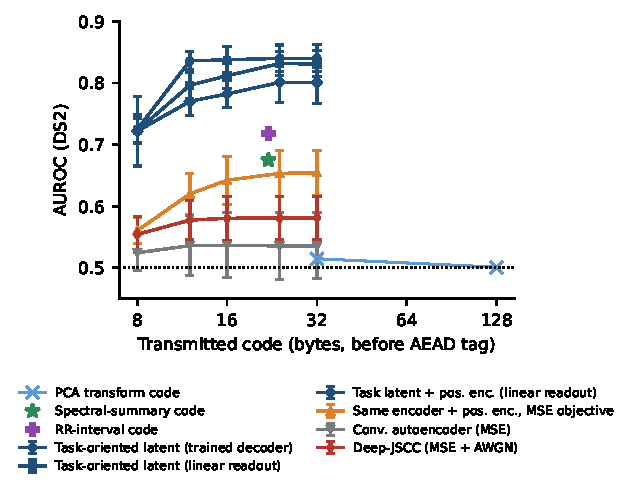
\includegraphics[width=\columnwidth]{figs/fig_proof.pdf}
\caption{AUROC on DS2 against transmitted code size (mean $\pm$ SD over seeds). Learned codecs share the 32-coefficient bottleneck and vary $b$; linear codes vary their coefficient count. The task-trained latent dominates at every payload and the reconstruction codecs stay near chance.}
\label{fig:proof}
\end{figure}
Table~\ref{tab:proof} and Fig.~\ref{fig:proof} hold the classifier fixed and vary only the representation. At 16 bytes the task-trained latent reaches \taskNativeSixteen{} with its trained decoder and \taskLogregSixteen{} with a linear readout, and it loses nothing between 32 and 12 bytes. The reconstruction codecs, trained for 60 epochs with validation-based selection and quantized after per-coefficient scaling, stay close to chance: \convaeSixteen{} for the convolutional autoencoder and \jsccSixteen{} for the deep-JSCC autoencoder at 16 bytes, with no dependence on $b$. \ifhavepe The symmetric pair isolates the objective with the architecture held fixed: with sinusoidal positional encodings added to both members, the task objective gives \taskPeSixteen{} under the same linear readout and the reconstruction objective \sameencSixteen{}---the identical network retains far more decision-relevant information per byte when trained for the decision, and the reconstruction-trained copy, although better than the convolutional autoencoder, remains closer to the hand-crafted codes than to the task code. (Positional encodings slightly lower the task model itself, \mainPeAUROC{} with its trained decoder against \mainAUROC{} without them, consistent with beat phase being a nuisance variable for this decision.) \fi Table~\ref{tab:recon} shows what the reconstruction codecs achieve on their own objective: at a 78:1 compression ratio on unaligned 10-s windows they reach PRDs of \convaePRD{}\% (convolutional autoencoder), \jsccPRD{}\% (deep JSCC)\ifhavepe, and \sameencPRD{}\% (task encoder with positional encodings)\fi{} on DS2, i.e.\ they reproduce little more than the window mean, although their training MSE is far lower (0.5--0.7), so the limit is generalization to unseen patients rather than optimization. Waveform reconstruction at this payload is not a viable objective, and whatever diagnostic content a reconstruction code retains is incidental. PCA (\pcaThirtyTwo{} at 32 coefficients, \pcaOneTwentyEight{} at 128) fails because beats are not phase-aligned across windows; the hand-crafted spectral code reaches \summaryProof{} and the RR-interval code \rrProof{}, both well below the learned task code but well above the reconstruction codes, because they are built for the decision. An earlier version of this comparison trained the autoencoders for six epochs and quantized their unscaled codes; the longer schedule and the scaling change the baseline numbers by a few hundredths and none of the conclusions. What a byte carries is set by what the code was trained to preserve.

\subsection{Ablation}\label{sec:ablation}
\begin{table}[!t]
\centering
\caption{Ablation on the de Chazal protocol (10 seeds). MACs are per 10-s window at 125 Hz, two leads, including attention.}
\label{tab:ablation}
\small
\resizebox{\columnwidth}{!}{\begin{tabular}{lcccrr}
\toprule
Variant & AUROC & Macro-F1 & Sens.@90\%Spec. & Enc. params & MACs/window \\
\midrule
Full model (CNN + 2-layer Transformer, all loss terms) & 0.835 $\pm$ 0.041 & 0.567 $\pm$ 0.018 & 0.726 $\pm$ 0.082 & 42,483 & 11,113,504 \\
CNN only (Transformer removed) & 0.809 $\pm$ 0.036 & 0.514 $\pm$ 0.039 & 0.666 $\pm$ 0.094 & 4,563 & 593,248 \\
One Transformer layer & 0.826 $\pm$ 0.023 & 0.574 $\pm$ 0.038 & 0.749 $\pm$ 0.054 & 23,523 & 5,853,376 \\
No latent $\ell_2$ term ($\lambda=0$) & 0.816 $\pm$ 0.046 & 0.556 $\pm$ 0.060 & 0.721 $\pm$ 0.096 & 42,483 & 11,113,504 \\
No rate term ($\gamma=0$) & 0.821 $\pm$ 0.038 & 0.563 $\pm$ 0.027 & 0.683 $\pm$ 0.097 & 42,483 & 11,113,504 \\
No early-exit head & 0.810 $\pm$ 0.052 & 0.549 $\pm$ 0.040 & 0.683 $\pm$ 0.092 & 42,483 & 11,113,504 \\
Task loss only & 0.780 $\pm$ 0.104 & 0.460 $\pm$ 0.136 & 0.553 $\pm$ 0.348 & 42,483 & 11,113,504 \\
\bottomrule
\end{tabular}
}
\end{table}
Table~\ref{tab:ablation} removes one component at a time. The CNN-only encoder (Transformer removed, mean-pooled convolutional tokens) reaches \cnnAUROC{} with \cnnMACs{}\,M MACs and \cnnParams{} parameters, against \mainAUROC{} and \mainMACs{}\,M MACs for the full model; one Transformer layer gives \tfoneAUROC{}. Removing the latent $\ell_2$ term (\noregAUROC{}), the rate term (\norateAUROC{}), or the early-exit head (\noeeAUROC{}) individually lowers the mean by one to two hundredths, within the seed spread, whereas training with the task loss alone is unstable (\taskonlyAUROC{}, with three of ten seeds below 0.70): the auxiliary terms act jointly as regularizers that keep the latent inside the quantizer range and stabilize the six-epoch schedule rather than as sources of accuracy. The Transformer accounts for the accuracy margin over the CNN and for 95\% of the computation, a trade that Section~\ref{sec:energy} prices.

\subsection{Leads and sampling rate}\label{sec:input}
\begin{table}[!t]
\centering
\caption{Input configuration (de Chazal protocol, 10 seeds each).}
\label{tab:input}
\small
\resizebox{\columnwidth}{!}{\begin{tabular}{lccccrr}
\toprule
Input & Raw bytes/window & AUROC & Macro-F1 & Sens.@90\%Spec. & Tokens $L$ & MACs/window \\
\midrule
MLII only, 125 Hz & 2500 & 0.833 $\pm$ 0.041 & 0.572 $\pm$ 0.066 & 0.808 $\pm$ 0.082 & 157 & 11,043,504 \\
Two leads, 125 Hz & 5000 & 0.835 $\pm$ 0.041 & 0.567 $\pm$ 0.018 & 0.726 $\pm$ 0.082 & 157 & 11,113,504 \\
Two leads, 250 Hz & 10000 & 0.811 $\pm$ 0.051 & 0.533 $\pm$ 0.044 & 0.733 $\pm$ 0.132 & 313 & 31,531,008 \\
Two leads, 360 Hz (native) & 14400 & 0.776 $\pm$ 0.038 & 0.529 $\pm$ 0.045 & 0.698 $\pm$ 0.127 & 450 & 57,169,680 \\
\bottomrule
\end{tabular}
}
\end{table}
The design is single- or multi-lead: $C$ only changes the stem. Table~\ref{tab:input} shows that the wearable-relevant single-lead configuration (MLII only) reaches \mliiAUROC{}, so a one-electrode-pair patch loses little against the two-lead reference. The 125~Hz operating rate is below the 250--500~Hz recommended for diagnostic 12-lead morphology \cite{kligfield2007} but is common in ambulatory and heart-rate-variability use \cite{kwon2018}; retraining the same architecture at 250~Hz (\fsTwoFiftyAUROC{}) and at the native 360~Hz (\fsThreeSixtyAUROC{}) does not improve the AAMI window decision---it is slightly worse with the fixed model size and schedule, because the token sequence lengthens to 313 and 450 and the receptive field of each token shrinks in seconds---while the cost rises to \fsTwoFiftyMACs{}\,M and \fsThreeSixtyMACs{}\,M MACs because attention grows quadratically in $L$. For the beat-class decision studied here, 125~Hz loses nothing measurable and is the low-energy operating point; tasks that depend on fine QRS morphology would need to re-examine this choice.

\subsection{Quantization}\label{sec:quant}
\begin{table}[!t]
\centering
\caption{Rate--fidelity on DS2 (10 seeds): post-training quantization of the 8-bit-trained codec versus quantization-aware training at the target width.}
\label{tab:quant}
\small
\resizebox{\columnwidth}{!}{\begin{tabular}{cccccc}
\toprule
Bits/coeff.\ $b$ & Code (B) & Payload incl.\ AEAD (B) & PTQ AUROC & QAT AUROC & PTQ Macro-F1 \\
\midrule
8 & 32 & 60 & 0.835 $\pm$ 0.041 & (same model) & 0.567 $\pm$ 0.018 \\
6 & 24 & 52 & 0.835 $\pm$ 0.041 & -- & 0.567 $\pm$ 0.018 \\
4 & 16 & 44 & 0.834 $\pm$ 0.041 & 0.831 $\pm$ 0.034 & 0.568 $\pm$ 0.019 \\
3 & 12 & 40 & 0.832 $\pm$ 0.038 & 0.812 $\pm$ 0.047 & 0.567 $\pm$ 0.017 \\
2 & 8 & 36 & 0.721 $\pm$ 0.049 & -- & 0.521 $\pm$ 0.065 \\
8 ($D$=8, trained with 8 coeff., 5 seeds) & 8 & 36 & 0.829 $\pm$ 0.018 & -- & 0.572 $\pm$ 0.020 \\
8 ($D$=4, trained with 4 coeff.) & 4 & 32 & 0.829 $\pm$ 0.029 & -- & 0.552 $\pm$ 0.029 \\
\bottomrule
\end{tabular}
}
\end{table}
\begin{figure}[!t]
\centering
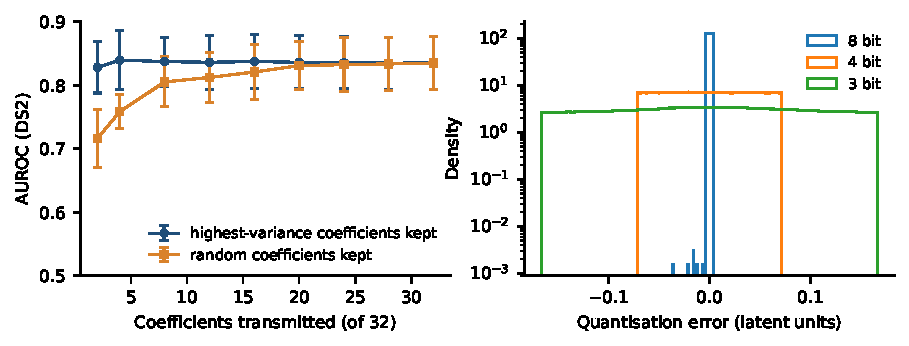
\includegraphics[width=\columnwidth]{figs/fig_quant.pdf}
\caption{Left: AUROC on DS2 when only $k$ of the 32 coefficients are transmitted (the rest set to zero), choosing the $k$ highest-variance coefficients of the training latent or $k$ random ones; mean and SD over 10 seeds. Right: distribution of the quantization error at 8, 4, and 3 bits pooled over seeds and coefficients.}
\label{fig:quant}
\end{figure}
Table~\ref{tab:quant} gives the rate--fidelity curve. Post-training requantization of the 8-bit-trained codec is lossless down to 3 bits (\ptqSix{} at 6 bits, \ptqFour{} at 4 bits, \ptqThree{} at 3 bits, i.e.\ a 12-byte code and 40-byte payload) and collapses only at 2 bits (\ptqTwo{}). Quantization-aware training at the target width does not help: \qatFour{} at 4 bits and \qatThree{} at 3 bits, slightly below PTQ, because the coarser straight-through quantizer adds gradient noise to a short schedule. One 8-bit model with post-hoc requantization is therefore the rate control, and the 4-bit quantization error (close to uniform, latent-to-error power ratio \snrFour{}~dB; Fig.~\ref{fig:quant}, right) is simply below what the decision needs. Fig.~\ref{fig:quant} (left) probes the second rate axis, the number of coefficients: erasing any single coefficient costs at most \dimMaxDrop{} AUROC, and keeping only the two or four highest-variance coefficients of the training latent (a 2- or 4-byte code) retains \subTopTwo{} and \subTopFour{}, whereas four random coefficients retain \subRandFour{}. The decision-relevant information thus occupies a few directions of a code whose variance is spread over about \kNinety{} coefficients, a redundancy the rate term does not remove. \ifhavelat \latConfirmSentence{} \fi At that point the 28-byte authentication tag and nonce, not the semantic code, set the payload, which turns the security layer into the dominant per-decision cost (Section~\ref{sec:security}).

\subsection{Channel robustness}\label{sec:channel}
\begin{figure*}[!t]
\centering
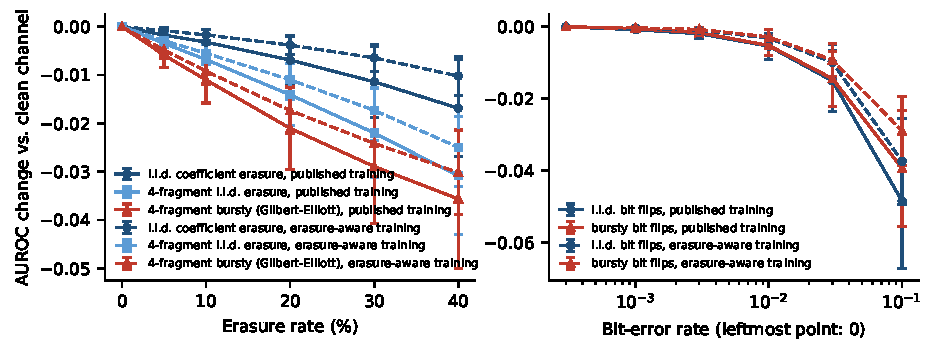
\includegraphics[width=0.8\textwidth]{figs/fig_channel.pdf}
\caption{Robustness on DS2 (10 seeds, 10 channel draws each). Left: coefficient and fragment erasures, i.i.d.\ and bursty. Right: bit flips on the 8-bit two's-complement code, i.i.d.\ and bursty. Solid: the published training; dashed: erasure-aware training.}
\label{fig:channel}
\end{figure*}
Fig.~\ref{fig:channel} reports the paired change in AUROC relative to each seed's clean channel, which removes the seed spread. Fidelity falls smoothly under erasure: at 40\% i.i.d.\ coefficient erasure the codec retains \iidForty{} (a drop of about 0.02), at 40\% i.i.d.\ fragment erasure \fragForty{}, and under the bursty fragment channel with the same mean loss \burstForty{}; fragment and bursty losses hurt more than scattered coefficient losses because a lost fragment can contain the few informative coefficients identified in Section~\ref{sec:quant}, which suggests interleaving them across fragments. Bit errors are tolerated up to a rate of $10^{-3}$ and cost about 0.005 at $10^{-2}$ (\bscOnePct{}) but 0.05 at $10^{-1}$ (\bscTenPct{}); the bursty bit-flip channel with the same mean rate is marginally kinder because errors concentrate in few coefficients. Erasure-aware training (dashed) leaves the clean-channel AUROC unchanged (\eraseZero{}) and roughly halves the loss under i.i.d.\ erasure (\eraseIidForty{} at 40\%), with a smaller gain under bursty fragment loss (\eraseBurstForty{}) and none against bit flips, for which the record layer's integrity check would in practice discard the packet. In a body-area deployment the relevant regime is packet erasure with ARQ, which the energy model prices next; the erasure curves say that a decision survives a lost fragment.

\subsection{Airtime and energy}\label{sec:energy}
\begin{table*}[!t]
\centering
\caption{Analytical per-decision costs (Section~\ref{sec:energymethod}; model-based, not measured). $E_{\rm tx}$ from datasheet currents; $E_{\rm cpu}$ from the MAC count at three INT8 throughputs; life for a 220-mAh cell at one decision per 10~s counting active energy only.}
\label{tab:energy}
\footnotesize
\resizebox{\textwidth}{!}{\begin{tabular}{llrrrrrr}
\toprule
Radio & Scheme (encoder, INT8 throughput) & Bytes & $E_\mathrm{tx}$ (mJ) & $E_\mathrm{cpu}$ (mJ) & Total (mJ) & Airtime (ms) & Life (d) \\
\midrule
BLE 1M (nRF52840) & Raw window & 5000 & 1.321 & 0 & 1.321 & 45.6 & 208 \\
 & Full codec, 40 MMAC/s & 60 & 0.026 & 2.751 & 2.776 & 0.88 & 99 \\
 & Full codec, 100 MMAC/s & 60 & 0.026 & 1.100 & 1.126 & 0.88 & 244 \\
 & Full codec, 200 MMAC/s & 60 & 0.026 & 0.550 & 0.576 & 0.88 & 478 \\
 & CNN-only codec, 40 MMAC/s & 60 & 0.026 & 0.147 & 0.172 & 0.88 & 1595 \\
 & CNN-only codec, 100 MMAC/s & 60 & 0.026 & 0.059 & 0.084 & 0.88 & 3263 \\
 & CNN-only codec, 200 MMAC/s & 60 & 0.026 & 0.029 & 0.055 & 0.88 & 5009 \\
\midrule
802.15.4 (CC2652R) & Raw window & 5000 & 13.660 & 0 & 13.660 & 189.7 & 20 \\
 & Full codec, 40 MMAC/s & 60 & 0.197 & 2.751 & 2.948 & 2.74 & 93 \\
 & Full codec, 100 MMAC/s & 60 & 0.197 & 1.100 & 1.298 & 2.74 & 212 \\
 & Full codec, 200 MMAC/s & 60 & 0.197 & 0.550 & 0.748 & 2.74 & 368 \\
 & CNN-only codec, 40 MMAC/s & 60 & 0.197 & 0.147 & 0.344 & 2.74 & 799 \\
 & CNN-only codec, 100 MMAC/s & 60 & 0.197 & 0.059 & 0.256 & 2.74 & 1074 \\
 & CNN-only codec, 200 MMAC/s & 60 & 0.197 & 0.029 & 0.227 & 2.74 & 1213 \\
\bottomrule
\end{tabular}
}
\end{table*}
\begin{figure}[!t]
\centering
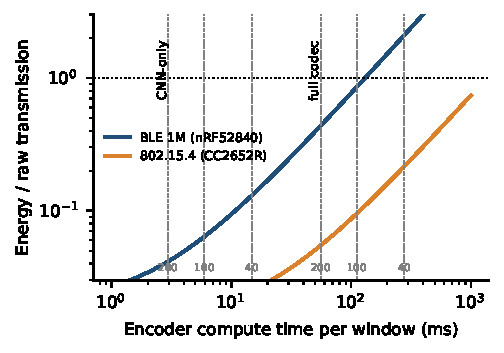
\includegraphics[width=\columnwidth]{figs/fig_energy.pdf}
\caption{Per-decision energy relative to raw transmission versus encoder compute time per window, for the two radios. Vertical lines mark the full and CNN-only codecs at 40, 100, and 200~M~MAC/s (right to left). Above the dotted line the encoder costs more than the radio bytes it saves.}
\label{fig:energy}
\end{figure}
The payload reduction is radio-agnostic: 60 bytes instead of 5000 cuts BLE airtime from \bleAirRaw{} to \bleAirSem{}~ms per decision (\airFactor$\times$), which lowers channel occupancy and collision probability on a shared band irrespective of energy. Energy is not radio-agnostic (Table~\ref{tab:energy}, Fig.~\ref{fig:energy}). On BLE, raw transmission costs \bleRaw{}~mJ, and the full codec's \mainMACs{}\,M MACs cost \bleFullForty{}~mJ at 40~M~MAC/s, \bleFullHundred{}~mJ at 100 and \bleFullTwoHundred{}~mJ at 200~M~MAC/s: the compute--radio crossover lies near \crossMMAC{}~M~MAC/s, i.e.\ about \cpuCrossBLEms{}~ms of Cortex-M4F compute per window, and the full codec saves energy on BLE only with optimized INT8 kernels. On IEEE~802.15.4, where a raw window costs \zRaw{}~mJ, the full codec saves \zFullFortyFactor$\times$ even at 40~M~MAC/s. The CNN-only codec of Section~\ref{sec:ablation} changes the picture: at \cnnMACs{}\,M MACs it costs \bleCnnForty{}~mJ on BLE and \zCnnForty{}~mJ on 802.15.4 at the conservative throughput, savings of \bleCnnFactor$\times$ and \zCnnFactor$\times$, while giving up the accuracy margin of Table~\ref{tab:ablation}. Under packet loss with retransmission the advantage of both codecs widens because the 5000-byte window spans 21 BLE or 44 IEEE~802.15.4 packets and pays the retransmission cost on each. The green conclusion is therefore conditional and explicit: task-oriented coding always buys airtime; it buys energy when the radio is slow, when the link is lossy, or when the encoder is kept at the CNN-only cost, and a Transformer head on an efficient radio must be justified by accuracy rather than by energy. An earlier version of this analysis, using a MAC count that omitted attention, overstated the BLE saving.

\subsection{Security overhead}\label{sec:security}
\begin{table}[!t]
\centering
\caption{Post-quantum-ready layer: standardized sizes \cite{fips203,fips204} and node-side cost from pqm4 Cortex-M4 cycle counts \cite{pqm4} at 64~MHz and 9.9~mW.}
\label{tab:sec}
\footnotesize
\resizebox{\columnwidth}{!}{\begin{tabular}{lrrr}
\toprule
Element & Bytes & Time (ms) & Energy (mJ) \\
\midrule
ML-KEM-512 encapsulation key (node $\to$ gateway) & 800 & -- & -- \\
ML-KEM-512 ciphertext (gateway $\to$ node) & 768 & -- & -- \\
ML-DSA-44 signature (gateway $\to$ node) & 2420 & -- & -- \\
ML-DSA-44 public key (provisioned once) & 1312 & -- & -- \\
Node: ML-KEM-512 key generation & -- & \pqKeygenMs & 0.06 \\
Node: ML-KEM-512 decapsulation & -- & \pqDecapsMs & 0.07 \\
Node: ML-DSA-44 verification & -- & \pqVerifyMs & 0.22 \\
Handshake total per session (node compute) & 3988 & \pqNodeMs & \pqNodeMJ \\
\midrule
AES-128-GCM tag + nonce, per decision & 28 & $<0.01$ & $<10^{-3}$ \\
\bottomrule
\end{tabular}}
\end{table}
Table~\ref{tab:sec} costs the layer of Section~\ref{sec:secmethod}. The one-time handshake moves about 4~kB per session (5.3~kB if the gateway's public key is re-sent rather than provisioned) and costs the node about \pqNodeMs~ms and \pqNodeMJ~mJ of computation---less than the radio energy of a single raw BLE window---and amortizes to under 1~byte/s after the first minute at a 10-s cadence. Steady-state security is the 28-byte tag and nonce already inside the 60-byte payload, and AES-GCM of 32 bytes is negligible on a Cortex-M4. Because the semantic code can shrink to 4--12 bytes (Section~\ref{sec:quant}), the fixed 28-byte overhead then dominates the packet; a 64-bit tag and an implicit sequence-number nonce, as permitted for constrained links, would halve the payload again, and the trade between tag length and forgery probability is the next design lever. A software implementation of the layer (kyber-py, dilithium-py, and the \texttt{cryptography} AES-GCM binding) reproduces the standardized sizes exactly; the cycle counts are pqm4's m4f measurements on a Cortex-M4 at 24~MHz scaled to 64~MHz, not on-target measurements of this system.

\subsection{Transfer to other data and modalities}
\begin{table}[!t]
\centering
\caption{Transfer beyond MIT-BIH with the unchanged architecture (five seeds\ifhaveptbxl; PTB-XL: \ptbxlNrec{} records on the official folds\fi).}
\label{tab:transfer}
\footnotesize
\resizebox{\columnwidth}{!}{\begin{tabular}{lccc}
\toprule
Dataset / task & AUROC & AUPRC & Macro-F1 \\
\midrule
\ptbxlRow
WESAD stress, chest ECG only & 0.823 $\pm$ 0.122 & -- & 0.710 $\pm$ 0.131 \\
WESAD stress, wrist PPG only & 0.951 $\pm$ 0.024 & -- & 0.843 $\pm$ 0.039 \\
WESAD stress, ECG + PPG & 0.867 $\pm$ 0.088 & -- & 0.756 $\pm$ 0.099 \\
\bottomrule
\end{tabular}}
\end{table}
\ifhaveptbxl Table~\ref{tab:transfer} extends the earlier 3039-record PTB-XL subset to the full database (\ptbxlNrec{} records with a diagnostic superclass, ten records whose signal files could not be read being excluded: \ptbxlNtrain{} training, \ptbxlNval{} validation, and \ptbxlNtest{} test on the official folds): the unchanged encoder, with twelve input channels and no tuning, separates normal from abnormal 12-lead recordings at an AUROC of \ptbxlAUROC{}. \else Table~\ref{tab:transfer} reports transfer to PTB-XL on a 3039-record subset drawn with the official stratified folds (2460 training, 285 validation, 294 test records): the unchanged encoder, with twelve input channels and no tuning, separates normal from abnormal 12-lead recordings at an AUROC of 0.890 $\pm$ 0.011; a run on all 21,799 records is in progress and will replace this subset result. \fi On WESAD the encoder processes chest ECG and wrist PPG alone and fused; PPG carries the strongest stress signal and fusion does not exceed it with this small architecture, but the experiment confirms multi-channel and cross-modality operation.

\section{Discussion and Limitations}\label{sec:discussion}
\textbf{What the results establish.} Coding for the decision rather than for the waveform is what makes a 60-byte payload sufficient: with \ifhavepe the same encoder, \fi the same classifier and equal training care, the reconstruction objective retains far less of the diagnostic information, and at this compression ratio it does not even reconstruct the waveform. The order-invariant latent is a compact description of \emph{which} local morphologies occur in a window, not \emph{where}, which is exactly the abstraction the AAMI decision needs. The bit-width is a single scalar control that trades payload against fidelity without retraining down to 3 bits, the decision survives the loss of most coefficients so that erasures and lost fragments degrade it gradually, and the node needs neither per-subject adaptation nor any protocol beyond encode--quantize--seal--send.

\textbf{What they do not establish.} Every energy and cryptographic figure is analytical. The energy model omits sleep and leakage currents, memory-access energy, sensor and analog front-end power, receive windows for acknowledgements, and connection maintenance, and it assumes a fixed INT8 throughput; the pqm4 cycle counts come from a different Cortex-M4 board and clock. These omissions affect both schemes and do not change the compute--radio crossover argument, which depends on ratios, but they do mean that Table~\ref{tab:energy} predicts rather than reports battery life. A microcontroller-and-radio testbed with current logging is the necessary next step, and the CNN-only codec is the variant to deploy first because its saving is robust to the throughput assumption.

\textbf{Data and task.} MIT-BIH is small and dates from the 1980s; the full PTB-XL run and the WESAD experiment broaden the evidence but use a single architecture and schedule, and absolute accuracy on DS2 remains moderate (AUROC \mainAUROC{}) with a seed spread that reflects the fixed 22-record test set. Supraventricular ectopy is the weak class for every representation, and signal-quality assessment, which a wearable pipeline needs to decide whether a window is worth transmitting at all, is a natural additional task head for the same latent. The channel models are abstractions of body-area links; binding the codec to a specific physical layer with a learned channel code, as in Deep-JSCC, remains open, although the erasure-aware variant shows that a latent-domain channel layer is straightforward to train.

\section{Conclusion}
A task-oriented semantic codec for wearable ECG was formulated end to end and evaluated as a green-communication design. On the inter-patient MIT-BIH protocol it reaches an AUROC of \mainAUROC{} with a 60-byte payload, retains \taskNativeSixteen{} at 16 bytes where \ifhavepe the same encoder trained for reconstruction retains \sameencSixteen{}\else reconstruction codecs of the same payload stay near chance\fi, tolerates 3-bit post-training quantization and 40\% bursty erasure with graceful loss, carries its decision in a handful of coefficients, and adds only 28 bytes of steady-state overhead for post-quantum-ready security, which then becomes the payload floor. The analytical energy model, corrected to count attention operations, shows that the payload saving always translates into airtime but into energy only when the radio is slow, the channel lossy, or the encoder kept at the CNN-only cost of \cnnMACs{}\,M MACs; on an efficient BLE radio the Transformer head must earn its place through accuracy. On-device measurement of these predictions is the immediate future work.

\begin{thebibliography}{99}
\bibitem{shannon1948} C. E. Shannon, ``A mathematical theory of communication,'' \emph{Bell Syst. Tech. J.}, vol. 27, no. 3, pp. 379--423, 1948.
\bibitem{strinati2021} E. C. Strinati and S. Barbarossa, ``6G networks: Beyond Shannon towards semantic and goal-oriented communications,'' \emph{Comput. Netw.}, vol. 190, Art. no. 107930, 2021.
\bibitem{gunduz2023} D. G\"und\"uz \emph{et al.}, ``Beyond transmitting bits: Context, semantics, and task-oriented communications,'' \emph{IEEE J. Sel. Areas Commun.}, vol. 41, no. 1, pp. 5--41, 2023.
\bibitem{qin2022} Z. Qin, X. Tao, J. Lu, W. Tong, and G. Y. Li, ``Semantic communications: Principles and challenges,'' arXiv:2201.01389, 2022.
\bibitem{yang2023} W. Yang \emph{et al.}, ``Semantic communications for future internet: Fundamentals, applications, and challenges,'' \emph{IEEE Commun. Surveys Tuts.}, vol. 25, no. 1, pp. 213--250, 2023.
\bibitem{luo2022} X. Luo, H.-H. Chen, and Q. Guo, ``Semantic communications: Overview, open issues, and future research directions,'' \emph{IEEE Wireless Commun.}, vol. 29, no. 1, pp. 210--219, 2022.
\bibitem{getu2024} T. M. Getu, G. Kaddoum, and M. Bennis, ``A survey on goal-oriented semantic communication: Techniques, challenges, and future directions,'' \emph{IEEE Access}, vol. 12, pp. 51223--51274, 2024.
\bibitem{bourtsoulatze2019} E. Bourtsoulatze, D. Burth Kurka, and D. G\"und\"uz, ``Deep joint source-channel coding for wireless image transmission,'' \emph{IEEE Trans. Cogn. Commun. Netw.}, vol. 5, no. 3, pp. 567--579, 2019.
\bibitem{xie2021} H. Xie, Z. Qin, G. Y. Li, and B.-H. Juang, ``Deep learning enabled semantic communication systems,'' \emph{IEEE Trans. Signal Process.}, vol. 69, pp. 2663--2675, 2021.
\bibitem{weng2021} Z. Weng and Z. Qin, ``Semantic communication systems for speech transmission,'' \emph{IEEE J. Sel. Areas Commun.}, vol. 39, no. 8, pp. 2434--2444, 2021.
\bibitem{chen2024} M. Chen, W. Saad, and C. Yin, ``Semantic communications for wearable and implantable health monitoring,'' \emph{IEEE J. Biomed. Health Inform.}, 2024.
\bibitem{bernstein2017} D. J. Bernstein and T. Lange, ``Post-quantum cryptography,'' \emph{Nature}, vol. 549, no. 7671, pp. 188--194, 2017.
\bibitem{alagic2022} G. Alagic \emph{et al.}, ``Status report on the third round of the NIST post-quantum cryptography standardization process,'' NIST, Gaithersburg, MD, USA, Tech. Rep. NISTIR 8413, 2022.
\bibitem{dai2022} J. Dai \emph{et al.}, ``Nonlinear transform source-channel coding for semantic communications,'' \emph{IEEE J. Sel. Areas Commun.}, vol. 40, no. 8, pp. 2300--2316, 2022.
\bibitem{kurka2020} D. B. Kurka and D. G\"und\"uz, ``DeepJSCC-f: Deep joint source-channel coding of images with feedback,'' \emph{IEEE J. Sel. Areas Inf. Theory}, vol. 1, no. 1, pp. 178--193, 2020.
\bibitem{tung2022} T.-Y. Tung, D. B. Kurka, M. Jankowski, and D. G\"und\"uz, ``DeepJSCC-Q: Constellation constrained deep joint source-channel coding,'' \emph{IEEE J. Sel. Areas Inf. Theory}, vol. 3, no. 4, pp. 720--731, 2022.
\bibitem{balle2017} J. Ball\'e, V. Laparra, and E. P. Simoncelli, ``End-to-end optimized image compression,'' in \emph{Proc. Int. Conf. Learn. Represent. (ICLR)}, 2017.
\bibitem{balle2018} J. Ball\'e, D. Minnen, S. Singh, S. J. Hwang, and N. Johnston, ``Variational image compression with a scale hyperprior,'' in \emph{Proc. ICLR}, 2018.
\bibitem{hannun2019} A. Y. Hannun \emph{et al.}, ``Cardiologist-level arrhythmia detection and classification in ambulatory electrocardiograms using a deep neural network,'' \emph{Nature Med.}, vol. 25, no. 1, pp. 65--69, 2019.
\bibitem{ribeiro2020} A. H. Ribeiro \emph{et al.}, ``Automatic diagnosis of the 12-lead ECG using a deep neural network,'' \emph{Nature Commun.}, vol. 11, Art. no. 1760, 2020.
\bibitem{moody2001} G. B. Moody and R. G. Mark, ``The impact of the MIT-BIH Arrhythmia Database,'' \emph{IEEE Eng. Med. Biol. Mag.}, vol. 20, no. 3, pp. 45--50, 2001.
\bibitem{goldberger2000} A. L. Goldberger \emph{et al.}, ``PhysioBank, PhysioToolkit, and PhysioNet: Components of a new research resource for complex physiologic signals,'' \emph{Circulation}, vol. 101, no. 23, pp. e215--e220, 2000.
\bibitem{strodthoff2021} N. Strodthoff, P. Wagner, T. Schaeffter, and W. Samek, ``Deep learning for ECG analysis: Benchmarks and insights from PTB-XL,'' \emph{IEEE J. Biomed. Health Inform.}, vol. 25, no. 5, pp. 1519--1528, 2021.
\bibitem{wagner2020} P. Wagner \emph{et al.}, ``PTB-XL, a large publicly available electrocardiography dataset,'' \emph{Sci. Data}, vol. 7, Art. no. 154, 2020.
\bibitem{aami2012} \emph{Testing and Reporting Performance Results of Cardiac Rhythm and ST Segment Measurement Algorithms}, ANSI/AAMI Standard EC57:2012, Assoc. Adv. Med. Instrum., Arlington, VA, USA, 2012.
\bibitem{dechazal2004} P. de Chazal, M. O'Dwyer, and R. B. Reilly, ``Automatic classification of heartbeats using ECG morphology and heartbeat interval features,'' \emph{IEEE Trans. Biomed. Eng.}, vol. 51, no. 7, pp. 1196--1206, 2004.
\bibitem{acharya2017} U. R. Acharya \emph{et al.}, ``A deep convolutional neural network model to classify heartbeats,'' \emph{Comput. Biol. Med.}, vol. 89, pp. 389--396, 2017.
\bibitem{kachuee2018} M. Kachuee, S. Fazeli, and M. Sarrafzadeh, ``ECG heartbeat classification: A deep transferable representation,'' in \emph{Proc. IEEE Int. Conf. Healthcare Inform. (ICHI)}, 2018, pp. 443--444.
\bibitem{mousavi2019} S. Mousavi and F. Afghah, ``Inter- and intra-patient ECG heartbeat classification for arrhythmia detection: A sequence to sequence deep learning approach,'' in \emph{Proc. IEEE ICASSP}, 2019, pp. 1308--1312.
\bibitem{yildirim2018} \"O. Yildirim, P. P\l awiak, R.-S. Tan, and U. R. Acharya, ``Arrhythmia detection using deep convolutional neural network with long duration ECG signals,'' \emph{Comput. Biol. Med.}, vol. 102, pp. 411--420, 2018.
\bibitem{xia2023} Y. Xia, Y. Xiong, and K. Wang, ``A transformer model blended with CNN and denoising autoencoder for inter-patient ECG arrhythmia classification,'' \emph{Biomed. Signal Process. Control}, vol. 86, Art. no. 105271, 2023.
\bibitem{essa2021} E. Essa and X. Xie, ``An ensemble of deep learning-based multi-model for ECG heartbeats arrhythmia classification,'' \emph{IEEE Access}, vol. 9, pp. 103452--103464, 2021.
\bibitem{yildirim2018c} \"O. Yildirim, R. San Tan, and U. R. Acharya, ``An efficient compression of ECG signals using deep convolutional autoencoders,'' \emph{Cogn. Syst. Res.}, vol. 52, pp. 198--211, 2018.
\bibitem{mamaghanian2011} H. Mamaghanian, N. Khaled, D. Atienza, and P. Vandergheynst, ``Compressed sensing for real-time energy-efficient ECG compression on wireless body sensor nodes,'' \emph{IEEE Trans. Biomed. Eng.}, vol. 58, no. 9, pp. 2456--2466, 2011.
\bibitem{pan1985} J. Pan and W. J. Tompkins, ``A real-time QRS detection algorithm,'' \emph{IEEE Trans. Biomed. Eng.}, vol. BME-32, no. 3, pp. 230--236, 1985.
\bibitem{frustaci2018} M. Frustaci, P. Pace, G. Aloi, and G. Fortino, ``Evaluating critical security issues of the IoT world: Present and future challenges,'' \emph{IEEE Internet Things J.}, vol. 5, no. 4, pp. 2483--2495, 2018.
\bibitem{hatzivasilis2018} G. Hatzivasilis, K. Fysarakis, I. Papaefstathiou, and C. Manifavas, ``A review of lightweight block ciphers,'' \emph{J. Cryptogr. Eng.}, vol. 8, no. 2, pp. 141--184, 2018.
\bibitem{fips203} \emph{Module-Lattice-Based Key-Encapsulation Mechanism Standard}, NIST FIPS 203, Aug. 2024, doi: 10.6028/NIST.FIPS.203.
\bibitem{fips204} \emph{Module-Lattice-Based Digital Signature Standard}, NIST FIPS 204, Aug. 2024, doi: 10.6028/NIST.FIPS.204.
\bibitem{bos2018} J. Bos \emph{et al.}, ``CRYSTALS-Kyber: A CCA-secure module-lattice-based KEM,'' in \emph{Proc. IEEE Eur. Symp. Security Privacy (EuroS\&P)}, 2018, pp. 353--367.
\bibitem{ducas2018} L. Ducas \emph{et al.}, ``CRYSTALS-Dilithium: A lattice-based digital signature scheme,'' \emph{IACR Trans. Cryptogr. Hardw. Embed. Syst.}, vol. 2018, no. 1, pp. 238--268, 2018.
\bibitem{pqm4} M. J. Kannwischer, R. Petri, J. Rijneveld, P. Schwabe, and K. Stoffelen, ``pqm4: Post-quantum crypto library for the ARM Cortex-M4,'' 2019--2025. [Online]. Available: \url{https://github.com/mupq/pqm4} (benchmarks.md, m4f implementations, accessed Sep. 2026).
\bibitem{gcm} M. Dworkin, \emph{Recommendation for Block Cipher Modes of Operation: Galois/Counter Mode (GCM) and GMAC}, NIST SP 800-38D, Nov. 2007.
\bibitem{hkdf} H. Krawczyk and P. Eronen, ``HMAC-based extract-and-expand key derivation function (HKDF),'' IETF RFC 5869, May 2010.
\bibitem{ieee802156} \emph{IEEE Standard for Local and Metropolitan Area Networks---Part 15.6: Wireless Body Area Networks}, IEEE Std 802.15.6-2012, 2012.
\bibitem{ieee802154} \emph{IEEE Standard for Low-Rate Wireless Networks}, IEEE Std 802.15.4-2020, 2020.
\bibitem{gomez2012} C. Gomez, J. Oller, and J. Paradells, ``Overview and evaluation of Bluetooth Low Energy: An emerging low-power wireless technology,'' \emph{Sensors}, vol. 12, no. 9, pp. 11734--11753, 2012.
\bibitem{ble53} \emph{Bluetooth Core Specification}, Version 5.3, Bluetooth SIG, Kirkland, WA, USA, Jul. 2021.
\bibitem{ullah2012} S. Ullah \emph{et al.}, ``A comprehensive survey of wireless body area networks,'' \emph{J. Med. Syst.}, vol. 36, no. 3, pp. 1065--1094, 2012.
\bibitem{cavallari2014} R. Cavallari, F. Martelli, R. Rosini, C. Buratti, and R. Verdone, ``A survey on wireless body area networks: Technologies and design challenges,'' \emph{IEEE Commun. Surveys Tuts.}, vol. 16, no. 3, pp. 1635--1657, 2014.
\bibitem{nrf52840} Nordic Semiconductor, ``nRF52840 Product Specification,'' v1.11, Trondheim, Norway, 2024. [Online]. Available: \url{https://docs.nordicsemi.com/bundle/ps_nrf52840/page/keyfeatures_html5.html}
\bibitem{cc2652r} Texas Instruments, ``CC2652R SimpleLink Multiprotocol 2.4 GHz Wireless MCU,'' Datasheet SWRS207F, Dallas, TX, USA, rev. Sep. 2021. [Online]. Available: \url{https://www.ti.com/lit/gpn/cc2652r}
\bibitem{han2016} S. Han, H. Mao, and W. J. Dally, ``Deep compression: Compressing deep neural networks with pruning, trained quantization and Huffman coding,'' in \emph{Proc. ICLR}, 2016.
\bibitem{jacob2018} B. Jacob \emph{et al.}, ``Quantization and training of neural networks for efficient integer-arithmetic-only inference,'' in \emph{Proc. IEEE/CVF CVPR}, 2018, pp. 2704--2713.
\bibitem{lai2018} L. Lai, N. Suda, and V. Chandra, ``CMSIS-NN: Efficient neural network kernels for Arm Cortex-M CPUs,'' arXiv:1801.06601, 2018.
\bibitem{banbury2021} C. Banbury \emph{et al.}, ``MLPerf Tiny benchmark,'' in \emph{Proc. NeurIPS Datasets Benchmarks Track}, 2021.
\bibitem{howard2017} A. G. Howard \emph{et al.}, ``MobileNets: Efficient convolutional neural networks for mobile vision applications,'' arXiv:1704.04861, 2017.
\bibitem{chollet2017} F. Chollet, ``Xception: Deep learning with depthwise separable convolutions,'' in \emph{Proc. IEEE CVPR}, 2017, pp. 1251--1258.
\bibitem{vaswani2017} A. Vaswani \emph{et al.}, ``Attention is all you need,'' in \emph{Proc. Adv. Neural Inf. Process. Syst. (NeurIPS)}, 2017, pp. 5998--6008.
\bibitem{bengio2013} Y. Bengio, N. L\'eonard, and A. Courville, ``Estimating or propagating gradients through stochastic neurons for conditional computation,'' arXiv:1308.3432, 2013.
\bibitem{tishby2015} N. Tishby and N. Zaslavsky, ``Deep learning and the information bottleneck principle,'' in \emph{Proc. IEEE Inf. Theory Workshop (ITW)}, 2015, pp. 1--5.
\bibitem{alemi2017} A. A. Alemi, I. Fischer, J. V. Dillon, and K. Murphy, ``Deep variational information bottleneck,'' in \emph{Proc. ICLR}, 2017.
\bibitem{kingma2015} D. P. Kingma and J. Ba, ``Adam: A method for stochastic optimization,'' in \emph{Proc. ICLR}, 2015.
\bibitem{gilbert1960} E. N. Gilbert, ``Capacity of a burst-noise channel,'' \emph{Bell Syst. Tech. J.}, vol. 39, no. 5, pp. 1253--1265, 1960.
\bibitem{elliott1963} E. O. Elliott, ``Estimates of error rates for codes on burst-noise channels,'' \emph{Bell Syst. Tech. J.}, vol. 42, no. 5, pp. 1977--1997, 1963.
\bibitem{kligfield2007} P. Kligfield \emph{et al.}, ``Recommendations for the standardization and interpretation of the electrocardiogram: Part I,'' \emph{Circulation}, vol. 115, no. 10, pp. 1306--1324, 2007.
\bibitem{kwon2018} O. Kwon \emph{et al.}, ``Electrocardiogram sampling frequency range acceptable for heart rate variability analysis,'' \emph{Healthc. Inform. Res.}, vol. 24, no. 3, pp. 198--206, 2018.
\bibitem{schmidt2018} P. Schmidt, A. Reiss, R. Duerichen, C. Marberger, and K. Van Laerhoven, ``Introducing WESAD, a multimodal dataset for wearable stress and affect detection,'' in \emph{Proc. ACM Int. Conf. Multimodal Interaction (ICMI)}, 2018, pp. 400--408.
\end{thebibliography}
\end{document}
